%MIT License
%
%Copyright (c) 2017 dinkoosmankovic
%
%Permission is hereby granted, free of charge, to any person obtaining a copy
%of this software and associated documentation files (the "Software"), to deal
%in the Software without restriction, including without limitation the rights
%to use, copy, modify, merge, publish, distribute, sublicense, and/or sell
%copies of the Software, and to permit persons to whom the Software is
%furnished to do so, subject to the following conditions:
%
%The above copyright notice and this permission notice shall be included in all
%copies or substantial portions of the Software.
%
%THE SOFTWARE IS PROVIDED "AS IS", WITHOUT WARRANTY OF ANY KIND, EXPRESS OR
%IMPLIED, INCLUDING BUT NOT LIMITED TO THE WARRANTIES OF MERCHANTABILITY,
%FITNESS FOR A PARTICULAR PURPOSE AND NONINFRINGEMENT. IN NO EVENT SHALL THE
%AUTHORS OR COPYRIGHT HOLDERS BE LIABLE FOR ANY CLAIM, DAMAGES OR OTHER
%LIABILITY, WHETHER IN AN ACTION OF CONTRACT, TORT OR OTHERWISE, ARISING FROM,
%OUT OF OR IN CONNECTION WITH THE SOFTWARE OR THE USE OR OTHER DEALINGS IN THE
%SOFTWARE.


    \documentclass[12pt]{article}
    \usepackage{amsfonts,amsmath,amssymb}
    \usepackage{amsmath,multicol,eso-pic}
    \usepackage[utf8]{inputenc}
    \usepackage[T1]{fontenc}
    \usepackage[left=2.00cm, right=2.00cm, top=2.00cm, bottom=2.00cm]{geometry}
    \usepackage{titlesec}
    \usepackage{enumerate}
    \usepackage{breqn}
    \usepackage{tikz}
    \usepackage{rotating}
    %\renewcommand{\wedge}{~}
    %\renewcommand{\neg}{\overline}
    \titleformat{\section}{\large}{\thesection.}{1em}{}
    
    
    % % % % % POPUNITE PODATKE
    
    \newcommand{\prezimeIme}{Mašović Haris}
    \newcommand{\brIndexa}{17993}
    \newcommand{\brZadace}{3}
    
    % % % % % 
    
    \begin{document}
    
    \thispagestyle{empty}
    \begin{center}
      \vspace*{1cm}

      \vspace*{2cm}
      {\huge \bf Zadaća \brZadace } \\
      \vspace*{1cm}
      {\Large \bf iz predmeta Matematička logika i teorija izračunljivosti}

      \vspace*{2cm}

      {\Large Prezime i ime: \prezimeIme} \\
      \vspace*{0.75cm}
      {\Large Br. indexa: \brIndexa}

      \vspace*{3cm}
      \renewcommand{\arraystretch}{1.75}
      \begin{tabular}{|c|c|}
    	\hline Zadatak & Bodovi \\
    	\hline 1 &  \\
    	\hline 2 &  \\
    	\hline 3 &  \\
    	\hline 4 &  \\
    	\hline 5 &  \\
    	\hline
     \end{tabular}

      \vfill


      {\large Elektrotehnički fakultet Sarajevo}

    \end{center}
    \newpage
    \thispagestyle{empty}
    
    
    % % % % % Rješenja zadataka
	\begin{enumerate}
		\item Rješenje zadatka
		\\
		
		* Ovaj izraz ćemo prvo minimizirati i proširiti u SDNF, pa onda primjeniti Quine-McCLuskey algoritam: \\
		
		\begin{equation*}
		    \overline{(\overline{D} \Rightarrow \overline{B})(A \vee B)} \Leftrightarrow [(C \Leftrightarrow \overline{B}) \veebar{} (\overline{C} \Leftrightarrow \overline{B})] =
		    \overline{D}B~\vee~\overline{A}~\overline{B} \Leftrightarrow 
		    (C \Leftrightarrow \overline{B})(\overline{\overline{C} \Leftrightarrow \overline{B}})~\vee~ (\overline{C \Leftrightarrow \overline{B}})(\overline{C} \Leftrightarrow \overline{B})	\\	 =\\  
		    
		    =~\overline{D}B~\vee~\overline{A}~\overline{B} \Leftrightarrow \overline{C}B~\vee~ \overline{B}C~\overline{C}~\vee~BC~\vee~\overline{B}C~=~\overline{D}B~\vee~\overline{A}~\overline{B} \Leftrightarrow \top~=~\overline{D}B~\vee~\overline{A}~\overline{B} 
		\end{equation*}
		\\
		
		* Proširujemo u SDNF: \\
		
		\begin{equation*}
		    ~\overline{D}B~\vee~\overline{A}~\overline{B} = ~\overline{A}~\overline{B}(D~\vee~\overline{D})(C~\vee~\overline{C})~\vee~B\overline{D}(A \vee \overline{A})(C \vee \overline{C}) = \\
		    
		    \overline{A}~\overline{B}~\overline{C}~\overline{D} \vee \overline{A}~\overline{B}~\overline{C}D \vee \overline{A}~\overline{B}C\overline{D} \vee \overline{A}~\overline{B}CD \vee \overline{A}B\overline{C}~\overline{D} \vee \overline{A}BC\overline{D} \vee AB\overline{C}~\overline{D} \vee ABC\overline{D} ~~~~ (SDNF)
		\end{equation*}
		\\
		
		* Sad prelazimo na QM-algoritam: \\
		
        \begin{tabular}{|c|c|c|c|}
        \hline0 & //             & //                  & //          \\
        \hline1 & ABC\overline{D}           & AB\overline{D}~~BC\overline{D}             & 
        B\overline{D}~\star ~~ B\overline{D}~\star       \\
        \hline 2 & AB\overline{C}~\overline{D} ~~ \overline{A}BC\overline{D}~~\overline{A}~\overline{B}CD & B\overline{C}~\overline{D} ~~ \overline{A}B\overline{D} ~~  \overline{A}C\overline{D} ~~ ~\overline{A}~\overline{B}C ~~ \overline{A}~\overline{B}D & \overline{A}~\overline{D}~\star  ~~ \overline{A}~\overline{B}~\star \\
        \hline 3 & \overline{A}B\overline{C}~\overline{D} ~~ \overline{A}~\overline{B}C\overline{D} ~~ \overline{A}~\overline{B}~\overline{C}D & \overline{A}~\overline{C}~\overline{D} ~~  \overline{A}~\overline{B}~\overline{D} ~~ \overline{A}~\overline{B}~\overline{C}         & //          \\
        \hline 4 & \overline{A}~\overline{B}~\overline{C}~\overline{D}           & //                  & //        \\
        \hline
        \end{tabular}
        \\
        
        ** Sve označene minterme sa {$\star$} su: \\   
        \begin{equation*}
            B\overline{D} \vee \overline{A}~\overline{D} \vee \overline{A}~\overline{B}
        \end{equation*}
		
		** Dalje formiramo tablicu pokrivanja da bi dobili naš MDNF: \\
		
		\begin{tabular}{|c|c|c|c|c|c|c|c|c|}
        \hline      & \overline{A}~\overline{B}~\overline{C}~\overline{D} & \overline{
        A}~\overline{B}~\overline{C}D & \overline{A}~\overline{B}C\overline{D} & \overline{A}~\overline{B}CD & \overline{A}B\overline{C}~\overline{D} & \overline{A}BC\overline{D} & AB\overline{C}~\overline{D} & ABC\overline{D} \\
        \hline B\overline{D} &      &      &      &      &  \star   &  \star    &  \star    & \star \\
        \hline \overline{A}~\overline{D}              &   \star   &      & \star     &      &  \star    & \star     &      &      \\
        \hline \overline{A}~\overline{B}             &  \star    & \star     & \star     & \star     &      &      &      &      \\
        \hline
        
        \end{tabular}
        \\
        
        *** Posmatrajući minterme u prvom i trećem redu možemo zaključiti da je to naš MDNF, odnosno:   
        \begin{equation*}
                B\overline{D} \vee \overline{A}~\overline{B}  ~~~ (MDNF)
        \end{equation*}
        \\
        ** Pošto imamo MDNF možemo izraziti taj izraz preko Šefer operacije dvostrukom negacijom: 
        \begin{equation*}
            \overline{\overline{B\overline{D}} \wedge \overline{\overline{A}~\overline{B}}} =~ \uparrow(\overline{B\overline{D}}, \overline{\overline{A}~\overline{B}}) = 
            \uparrow(\uparrow(B, D \uparrow D), \uparrow(\overline{A} \uparrow \overline{B})) = \uparrow(\uparrow(B, D \uparrow D), \uparrow(A \uparrow A, B \uparrow B)) \\
        \end{equation*}
        \newpage

        * Ukoliko negiramo naš SDNF i negiramo dobiti ćemo našu negaciju SKNF-a: \\
        
        \begin{equation*}
        
            \overline{\overline{A}~\overline{B}~\overline{C}~\overline{D} \vee \overline{A}~\overline{B}~\overline{C}D \vee \overline{A}~\overline{B}C\overline{D} \vee \overline{A}~\overline{B}CD \vee \overline{A}B\overline{C}~\overline{D} \vee \overline{A}BC\overline{D} \vee AB\overline{C}~\overline{D} \vee ABC\overline{D}} = \\
            
            = (A \vee B \vee C \vee D)(A \vee B \vee C \vee \overline{D})(A \vee B \vee \overline{C} \vee D)(A \vee B \vee \overline{C} \vee \overline{D})(A \vee \overline{B} \vee C \vee D)\\            
            (A \vee \overline{B} \vee \overline{C} \vee D)(\overline{A} \vee \overline{B} \vee \overline{C} \vee D)(\overline{A} \vee \overline{B} \vee C \vee D) = \\
            
            \overline{A}B\overline{C}D \vee \overline{A}BCD \vee A\overline{B}~\overline{C}~\overline{D} \vee A\overline{B}~\overline{C}~\overline{D} \vee A\overline{B}~\overline{C}D \vee A\overline{B}C\overline{D} \vee A\overline{B}CD \vee AB\overline{C}D \vee ABCD ~(*)
            
        \end{equation*}
        ** Dobiveni izraz (*) iznad predstavlja negaciju SKNF-a pomoću kojeg ćemo QM-algoritmom naći MDNF, pa taj dobiveni izraz negirati: \\
        
        \begin{tabular}{|c|c|c|c|}
        \hline 0 & ABCD           & ABD ACD BCD         & AD~\star ~~ BD~\star \\
        \hline 1 & AB\overline{C}D~~A\overline{B}CD~~\overline{A}BCD & B\overline{C}D~A\overline{C}D A\overline{B}D~A\overline{B}C~\overline{A}BD & A\overline{B}~\star    \\
        \hline 2 & \overline{A}B\overline{C}D~~A\overline{B}~\overline{C}~D A\overline{B}C\overline{D} & A\overline{B}~\overline{C}~~A\overline{B}~\overline{D}             & //    \\
        \hline 3 & A\overline{B}~\overline{C}~\overline{D}           & //                  & //    \\
        \hline 4 & //             & //                  & //    \\
        \hline
        \end{tabular}
        \\  
        ** Sve označene minterme sa {$\star$} su: \\
        \begin{equation*}
            AD \vee BD \vee A\overline{B}
        \end{equation*}
        ** Dalje formiramo tablicu pokrivanja da bi dobili naš MDNF pa negacijom MKNF: \\
        
        \begin{tabular}{|c|c|c|c|c|c|c|c|c|}
         \hline    & \overline{A}B\overline{C}D & \overline{A}BCD & A\overline{B}~\overline{C}~\overline{D} & A\overline{B}~\overline{C}D & A\overline{B}C\overline{D} & A\overline{B}CD & AB\overline{C}D & ABCD \\
         \hline AD &      &      &      & \star     &      & \star      & \star     & \star     \\
         \hline BD &   \star   & \star      &      &      &      &      &   \star   &  \star      \\
         \hline A\overline{B} &      &      &   \star   & \star     & \star     & \star     &      &    \\
         \hline
        \end{tabular}
        
        *** Vidimo da se AD može sažimati samim tim dobijamo naš privremeni MDNF koji glasi: \\
        \begin{equation*}
            BD \vee A\overline{B}
        \end{equation*}
        
        * I negacijom ovog izraza dobijamo naš MKNF: \\
        \begin{equation*}
            (\overline{B} \vee \overline{D})(\overline{A} \vee B)
        \end{equation*}
        
        ** Pošto imamo MKNF možemo izraziti taj izraz preko Pierce operacije dvostrukom negacijom: \\
        
        \overline{\overline{(\overline{B} \vee \overline{D})(\overline{A} \vee B)}} =~ \downarrow(\overline{\overline{B} \vee \overline{D}}, \overline{\overline{A} \vee B}) =~ \downarrow(\downarrow(B \downarrow B, D \downarrow D), \downarrow( A \downarrow A, B))
        
        \newpage
		\item Rješenje zadatka
		
		* Prvo ćemo naći SDNF našeg početnog izraza: \\
		\begin{equation*}
		    \overline{A}~\overline{B}~\overline{C} \vee ABC \vee AB\overline{C}~\overline{D} \vee ABD =
		    \overline{A}~\overline{B}~\overline{C}D \vee \overline{A}~\overline{B}~\overline{C}~\overline{D} \vee ABCD \vee ABC\overline{D} \vee AB\overline{C}~\overline{D} \vee AB\overline{C}D
		\end{equation*}
		
		** Dalje formiramo QM-algoritam uz predpostavku iz zadatka: \\
		
		\begin{tabular}{|c|c|c|c|}
        \hline 0 & ABCD      & ABC~~ABD~~BCD & AB \star ~~ BC \star \\
        \hline 1 & ABC\overline{D}~~AB\overline{C}D ~~ \overline{A}BCD & AB\overline{D}~~BC\overline{D}~~AB\overline{C}~~\overline{A}CD~~\overline{A}BC & \overline{A}C~(\star~\star) \\
        \hline 2 & AB\overline{C}~\overline{D}~~\overline{A}BC\overline{D}~~\overline{A}~\overline{B}CD      & \overline{A}C\overline{D}~~\overline{A}~\overline{B}D~~\overline{A}~\overline{B}C      & \overline{A}~\overline{B}~\star  \\
        \hline 3 & \overline{A}~\overline{B}~\overline{C}D~~\overline{A}~\overline{B}C\overline{D}    & \overline{A}~\overline{B}~\overline{C}~~ \overline{A}~\overline{B}~\overline{D}   & // \\
        \hline 4 & \overline{A}~\overline{B}~\overline{C}~\overline{D}      & //      & //  \\
        \hline 
        \end{tabular}
        
        ** Ukoliko formirano izraz samo sa {$\star$} imamo: \\
        \begin{equation*}
            AB \vee BC \vee \overline{A}~\overline{B}
        \end{equation*}
        
        ** Dalje formiramo tablicu pokrivanja da bi dobili naš MDNF: \\
		
		\begin{tabular}{|c|c|c|c|c|c|c|}
        \hline     & \overline{A}~\overline{B}~\overline{C}D & \overline{A}~\overline{B}~\overline{C}~\overline{D} & ABCD & ABC\overline{D} & AB\overline{C}~\overline{D} & AB\overline{C}D \\
        \hline AB  &      &      &  \star    & \star      & \star     & \star     \\
        \hline BC &      &     &  \star     &  \star     &      &   \\  
        \hline \overline{A}~\overline{B} & \star  & \star  & & & & \\
        \hline 
        \end{tabular}
        \\
        
        *** Vidimo da možemo još sažimati naš traženi MDNF, samim tim dobijamo sljedeći izraz koji je naš traženi MDNF: \\
        \begin{equation*}
            AB \vee \overline{A}~\overline{B}
        \end{equation*}
		
		\item Rješenje zadatka
		
		* Prvo ćemo napisati zadane minterme u postavci kojih ima 25: \\
		
		\begin{equation*}
		
		    000000 \vee~000001 \vee 000010 \vee 000011 \vee 001000 \vee 001001 \vee 001010 \vee \\
		    
		    001011 \vee~010100 \vee 010101 \vee 011001 \vee 011010 \vee 011011 \vee 011100 \vee \\
		    
		    101000 \vee~101001 \vee 110111 \vee 111000 \vee 111001 \vee 111010 \vee 111011 \vee \\
		    
		    111100 \vee~111101 \vee 111110 \vee 111111
		
		 \end{equation*}
		\newpage
		
		** Pristupimo traženju implikanti koje pokrivaju ovu zadanu formu i pristupimo MINI algoritmom: \\
		
		(1)~~~ 00\_0\_\_ \\
		(2)~~~ 00\_011 \\
		(3)~~~ 01010\_ \\
		(4)~~~ 0110\_1 \\
		(5)~~~ 01101\_ \\
		(6)~~~ 10100\_ \\
		(7)~~~ 1110\_\_ \\
		(8)~~~ 1111\_\_ \\
		(9)~~~ 11\_111 \\
		(10)~~ 011100 \\
		
		* Pristupimo ekspanziji: \\
		000000 -> (1)~~(odbacivanje 000001 i 000010 i 001000) \\
		000011 -> (2)~~(odbacivanje 001011) \\
		001010 -> (3)~~(odbacivanje 001011 i 010100 i 010101) \\
		011001 -> (4)~~(odbacivanje 011011) \\
		011010 -> (5)~~(nema odbacivanja) \\
		101000 -> (6)~~(odbacivanje 101001) \\
		110111 -> (9)~~(odbacivanje 111111) \\
		111000 -> (7)~~(odbacivanje 111001 i 111010 i 111011) \\
		111100 -> (8)~~(odbacivanje 111101 i 111110) \\
		011100 -> (10)~(nema odbacivanja) \\
		
		* Pristupimo redukciji: \\
		(2) -> NIL (pokriveno od strane (1) i (3)) \\
		
		* Pristupimo preoblikovanju: \\
		1. (7) -> 111\_\_\_ , (8) -> 11111\_ \\
		
		* Vidimo da imamo pokrivanje u narednim implikantama: \\
		\{ (1),(3),(4),(5),(6),(7),(8),(9),(10) \} \\
		
		** Ponavljanjem, tj. drugom iteracijom ekspanzije imamo: \\
		(8) -> (7) \\
		
		** Redukcijom: \\
		(9) -> 110111 \\
		
		** Vidimo da dalje preoblikovanje nije moguće raditi pa imamo konačno pokrivanje koje glasi: \\
		\{ (1),(3),(4),(5),(6),(7),(9),(10) \}
		
		\newpage
		\item Rješenje zadatka
		\\
		
		* Ukoliko prvo malo sredimo izraz imamo i formiramo Veitchov dijagram za traženje MDNF imamo: \\
		\begin{equation*}
		    \overline{A}~\overline{B}~\overline{C}~\overline{C} \vee B\overline{D(\overline{A} \vee C \vee \overline{D})} \vee A\overline{C} \vee A\overline{B}CD = \overline{A}~\overline{B}~\overline{C}~\overline{D} \vee B\overline{D} \vee AB\overline{C}D \vee \overline{A}C \vee A\overline{B}CD
		\end{equation*}
		
		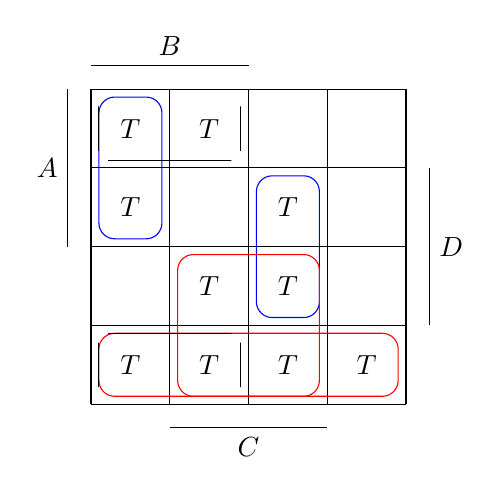
\begin{tikzpicture}
		\draw (0,0) grid (4,4);
		\node at (3.5,.5){ $T$ };
		\node at (3.5,1.5){ };
		\node at (2.5,0.5){ $T$ };
		\node at (2.5,1.5) { $T$ };
		\node at (.5,.5) { $T$ };
		\node at (.5,1.5){ };
		\node at (1.5,0.5){ $T$ };
		\node at (1.5,1.5){ $T$ };
		\node at (3.5,3.5){ };
		\node at (3.5,2.5){ };
		\node at (2.5,3.5){ };
		\node at (2.5,2.5){ $T$ };
		\node at (0.5,3.5){ $T$ };
		\node at (0.5,2.5){ $T$ };
		\node at (1.5,3.5){ $T$ };
		\node at (1.5,2.5){ };
		\draw (0,4.3) --node[midway, above]{$ B $} (2,4.3);
		\draw (-0.3,4) --node[midway, left]{$ A $} (-0.3,2);
		\draw (1,-0.3) --node[midway, below]{$ C $} (3,-0.3);
		\draw (4.3,1) --node[midway, right]{$ D $} (4.3,3);
		
		\draw [color=blue, rounded corners=2mm] (0.1, 3.9) -- (0.1, 2.1) -- (0.9, 2.1) -- (0.9, 3.9) -- cycle;
		\draw [color=blue, rounded corners=2mm] (2.1, 1.1) -- (2.1, 2.9) -- (2.9, 2.9) -- (2.9, 1.1) -- cycle;
		\draw [color=red, rounded corners=2mm] (1.1, 0.1) -- (1.1, 1.9) -- (2.9, 1.9) -- (2.9, 0.1) -- cycle;
		\draw [color=red, rounded corners=2mm] (0.1, 0.1) -- (0.1, 0.9) -- (3.9, 0.9) -- (3.9, 0.1) -- cycle;
		
		\draw [color=black, rounded corners=2mm] (0.1, 0.1) -- (0.1, 0.9) -- cycle;
		\draw [color=black, rounded corners=2mm] (0.1, 0.9) -- (1.9, 0.9) -- cycle;
		\draw [color=black, rounded corners=2mm] (1.9, 0.9) -- (1.9, 0.1) -- cycle;
		
		\draw [color=black, rounded corners=2mm] (0.1, 3.9) -- (0.1, 3.1) -- cycle;
		\draw [color=black, rounded corners=2mm] (0.1, 3.1) -- (1.9, 3.1) -- cycle;
		\draw [color=black, rounded corners=2mm] (1.9, 3.9) -- (1.9, 3.1) -- cycle;
	    \end{tikzpicture}
	    \\
	    \\
	    
	    ** Plavom bojom su označene esencijalne konture dok su crvenom i crnom konturom predstavljene ostale minterme, iz Veitchovog dijagrama možemo očitati naš MDNF, pri tome da su prve dvije minterme ove sa plavim konturama: \\
	    
	    \begin{equation*}
	        AB\overline{C} \vee \overline{B}CD \vee B\overline{D} \vee \overline{A}~\overline{D} \vee \overline{A}C ~~~~~~~~ (MDNF)
	    \end{equation*}
	    
	    * Dalje ukoliko ponovimo isti postupak, ali samo za MKNF (pri tome da u prazna polja uvrštavamo T) imamo: \\
	    
	    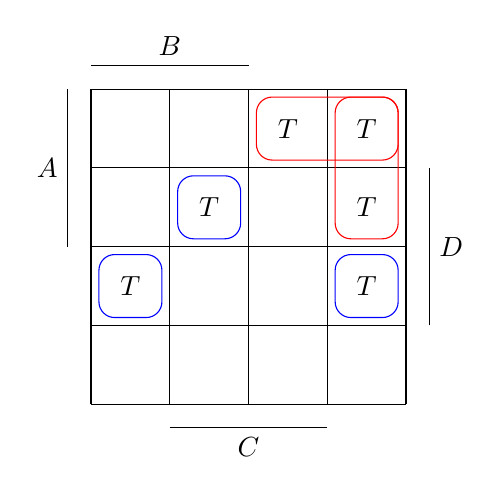
\begin{tikzpicture}
		\draw (0,0) grid (4,4);
		\node at (3.5,.5){ };
		\node at (3.5,1.5){ $T$ };
		\node at (2.5,0.5){ };
		\node at (2.5,1.5) { };
		\node at (.5,.5) { };
		\node at (.5,1.5){ $T$ };
		\node at (1.5,0.5){ };
		\node at (1.5,1.5){ };
		\node at (3.5,3.5){ $T$ };
		\node at (3.5,2.5){ $T$ };
		\node at (2.5,3.5){ $T$ };
		\node at (2.5,2.5){ };
		\node at (0.5,3.5){ };
		\node at (0.5,2.5){ };
		\node at (1.5,3.5){ };
		\node at (1.5,2.5){ $T$ };
		\draw (0,4.3) --node[midway, above]{$ B $} (2,4.3);
		\draw (-0.3,4) --node[midway, left]{$ A $} (-0.3,2);
		\draw (1,-0.3) --node[midway, below]{$ C $} (3,-0.3);
		\draw (4.3,1) --node[midway, right]{$ D $} (4.3,3);
		
		\draw [color=blue, rounded corners=2mm] (0.1, 1.1) -- (0.1, 1.9) -- (0.9, 1.9) -- (0.9, 1.1) -- cycle;
		\draw [color=blue, rounded corners=2mm] (1.1, 2.1) -- (1.1, 2.9) -- (1.9, 2.9) -- (1.9, 2.1) -- cycle;
		\draw [color=blue, rounded corners=2mm] (3.1, 1.1) -- (3.1, 1.9) -- (3.9, 1.9) -- (3.9, 1.1) -- cycle;
		\draw [color=red, rounded corners=2mm] (2.1, 3.1) -- (2.1, 3.9) -- (3.9, 3.9) -- (3.9, 3.1) -- cycle;
		\draw [color=red, rounded corners=2mm] (3.1, 2.1) -- (3.1, 3.9) -- (3.9, 3.9) -- (3.9, 2.1) -- cycle;
	\end{tikzpicture}

        ** Ukoliko posmatramo naše konture imamo da je naš MKNF: \\
        \begin{equation*}
            \overline{\overline{A}D\overline{C} \vee ABCD \vee A\overline{B}~\overline{D} \vee A\overline{B}~\overline{C}} = (A \vee \overline{D} \vee C)(\overline{A} \vee \overline{B} \vee \overline{C} \vee \overline{D})(\overline{A} \vee B \vee D)(\overline{A} \vee B \vee C)
        \end{equation*}
		\\
		
		*** Sada prelzimo na traženje MEXDNF našeg izraza: \\
		
		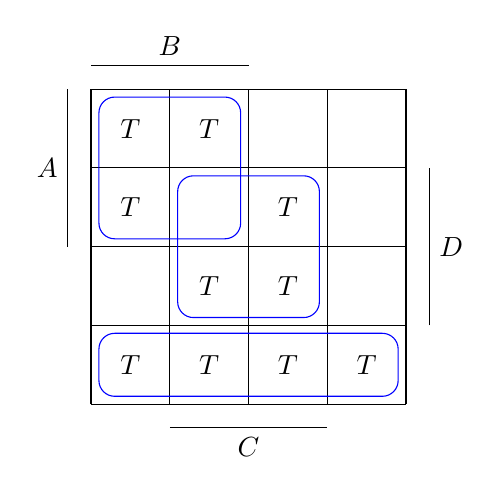
\begin{tikzpicture}
		\draw (0,0) grid (4,4);
		\node at (3.5,.5){ $T$ };
		\node at (3.5,1.5){ };
		\node at (2.5,0.5){ $T$ };
		\node at (2.5,1.5) { $T$ };
		\node at (.5,.5) { $T$ };
		\node at (.5,1.5){ };
		\node at (1.5,0.5){ $T$ };
		\node at (1.5,1.5){ $T$ };
		\node at (3.5,3.5){ };
		\node at (3.5,2.5){ };
		\node at (2.5,3.5){ };
		\node at (2.5,2.5){ $T$ };
		\node at (0.5,3.5){ $T$ };
		\node at (0.5,2.5){ $T$ };
		\node at (1.5,3.5){ $T$ };
		\node at (1.5,2.5){ };
		\draw (0,4.3) --node[midway, above]{$ B $} (2,4.3);
		\draw (-0.3,4) --node[midway, left]{$ A $} (-0.3,2);
		\draw (1,-0.3) --node[midway, below]{$ C $} (3,-0.3);
		\draw (4.3,1) --node[midway, right]{$ D $} (4.3,3);
		
		\draw [color=blue, rounded corners=2mm] (0.1, 0.1) -- (0.1, 0.9) -- (3.9, 0.9) -- (3.9, 0.1) -- cycle;
		\draw [color=blue, rounded corners=2mm] (0.1, 3.9) -- (0.1, 2.1) -- (1.9, 2.1) -- (1.9, 3.9) -- cycle;
		\draw [color=blue, rounded corners=2mm] (1.1, 1.1) -- (1.1, 2.9) -- (2.9, 2.9) -- (2.9, 1.1) -- cycle;
		\end{tikzpicture}
		
		*** Iz Veitchovog dijagrama možemo pročitati naš MEXDNF koji glasi: \\
		\begin{equation*}
		    \overline{A}~\overline{D} \veebar{} AB \veebar{} CD ~~~(MEXDNF)
		\end{equation*}
		
		\item Rješenje zadatka
		\\
		
		* Po postavci zadatka i zadatoj tabeli istine, može se zaključiti da trebamo posmatrati i dodatne 'zabranjene' kombinacije. I ukoliko uvedemo naredne oznake da je A = B1, B = B2, C = B3, D = B4, E = B5, na osnovu toga imamo sljedeći Veitchov dijagram: \\
		
		
        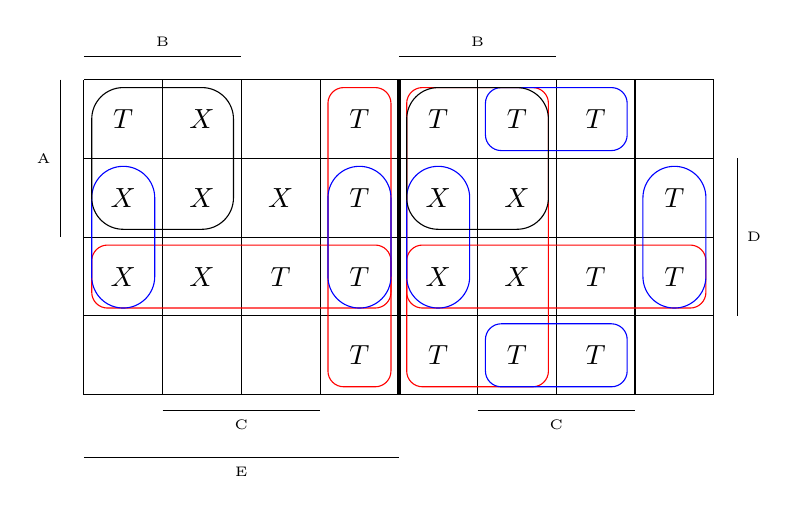
\begin{tikzpicture}
		\draw (0,0) grid (8,4);
		\node at (3.5,.5){ $T$  };
		\node at (3.5,1.5){ $T$  };
		\node at (2.5,0.5){ };
		\node at (2.5,1.5) { $T$ };
		\node at (.5,.5) { };
		\node at (.5,1.5){ $X$  };
		\node at (1.5,0.5){ };
		\node at (1.5,1.5){ $X$ };
		\node at (3.5,3.5){ $T$ };
		\node at (3.5,2.5){ $T$  };
		\node at (2.5,3.5){  };
		\node at (2.5,2.5){ $X$  };
		\node at (0.5,3.5){ $T$ };
		\node at (0.5,2.5){ $X$  };
		\node at (1.5,3.5){ $X$ };
		\node at (1.5,2.5){ $X$  };
		\node at (7.5,.5){  };
		\node at (7.5,1.5){  $T$ };
		\node at (6.5,0.5){ $T$ };
		\node at (6.5,1.5) { $T$ };
		\node at (4.5,.5) { $T$ };
		\node at (4.5,1.5){ $X$ };
		\node at (5.5,0.5){ $T$ };
		\node at (5.5,1.5){ $X$ };
		\node at (7.5,3.5){ };
		\node at (7.5,2.5){ $T$ };
		\node at (6.5,3.5){ $T$ };
		\node at (6.5,2.5){  };
		\node at (4.5,3.5){ $T$ };
		\node at (4.5,2.5){ $X$  };
		\node at (5.5,3.5){ $T$ };
		\node at (5.5,2.5){ $X$  };
		\draw (-0.3,4) --node[midway, left]{\tiny A} (-0.3,2);
		\draw (0,4.3) --node[midway, above]{\tiny B} (2,4.3);
		\draw (4,4.3) --node[midway, above]{\tiny B} (6,4.3);
		\draw (1,-0.2) --node[midway, below]{\tiny C} (3,-0.2);
		\draw (5,-0.2) --node[midway, below]{\tiny C} (7,-0.2);
		\draw (8.3,1) --node[midway, right]{\tiny D} (8.3,3);
		\draw (0,-0.8) --node[midway, below]{\tiny E} (4,-0.8);
		\draw [line width=0.5mm ] (4,0) -- (4,4);
		
		\draw [color=red, rounded corners=2mm] (3.1, 0.1) -- (3.1, 3.9) -- (3.9, 3.9) -- (3.9, 0.1) -- cycle;
		\draw [color=red, rounded corners=2mm] (0.1, 1.1) -- (0.1, 1.9) -- (3.9, 1.9) -- (3.9, 1.1) -- cycle;
		\draw [color=red, rounded corners=2mm] (4.1, 1.1) -- (4.1, 1.9) -- (7.9, 1.9) -- (7.9, 1.1) -- cycle;
		\draw [color=red, rounded corners=2mm] (4.1, 0.1) -- (4.1, 3.9) -- (5.9, 3.9) -- (5.9, 0.1) -- cycle;
		\draw [color=blue, rounded corners=2mm] (5.1, 0.1) -- (5.1, 0.9) -- (6.9, 0.9) -- (6.9, 0.1) -- cycle;
		\draw [color=blue, rounded corners=2mm] (5.1, 3.1) -- (5.1, 3.9) -- (6.9, 3.9) -- (6.9, 3.1) -- cycle;
		
		\draw [color=blue, rounded corners=4mm] (3.1, 1.1) -- (3.1, 2.9) -- (3.9, 2.9) -- (3.9, 1.1) -- cycle;
		\draw [color=blue, rounded corners=4mm] (7.1, 1.1) -- (7.1, 2.9) -- (7.9, 2.9) -- (7.9, 1.1) -- cycle;
		\draw [color=blue, rounded corners=4mm] (4.1, 1.1) -- (4.1, 2.9) -- (4.9, 2.9) -- (4.9, 1.1) -- cycle;
		\draw [color=blue, rounded corners=4mm] (0.1, 1.1) -- (0.1, 2.9) -- (0.9, 2.9) -- (0.9, 1.1) -- cycle;
		
		\draw [color=black, rounded corners=4mm] (0.1, 2.1) -- (0.1, 3.9) -- (1.9, 3.9) -- (1.9, 2.1) -- cycle;
		\draw [color=black, rounded corners=4mm] (4.1, 2.1) -- (4.1, 3.9) -- (5.9, 3.9) -- (5.9, 2.1) -- cycle;
		
	\end{tikzpicture}
		
	*** Iz Veitchovog dijagrama možemo zaključiti da rješenje traženo je: \\
	\begin{equation*}
	    B\overline{E} \vee C\overline{D}~\overline{E} \vee \overline{A}D \vee \overline{B}~\overline{C}~E \vee AB \vee \overline{C}D
	\end{equation*}
		
		
	\end{enumerate}
	
	
	
    \end{document}
    